\section{Continuous and Discrete Actions Spaces}
The difference between discrete and continuous actions spaces has been pointed out in the paragraphs about the policy gradients methods of the \ref{Solution Methods} section, where the discrete policy operation is described and where the components of the continuous policy are explained and, also in the \ref{ANNstructure} section, where the ANN structure in Figure \ref{A3CTorcs} illustrates the contrast in the policy formation of both actions spaces.

No matter the problem, the actions are declared depending on the requirements of the environment that it is being worked with. In TORCS, the action of steering, for example, is always a number between -1 and +1.

The discrete policy estimates the probabilities of taking each possible action in a clearly identified state. Therefore, a set of pre-defined actions should be declared. For instance, a choice for representing the steering action is to divide it into three parts, one action for steering in the left direction with the value +1, another action for not making any changes with the value 0, and an action for steering in the right direction with the value -1. This results in 3 actions, just to represent the steering. When the discrete policy layer assigns probabilities for each of these actions, the action with the highest probability is then deployed in the environment.

The results of training for a single action - steering, are present at the beginning of this chapter in the figures \ref{fig:Length}, \ref{fig:Reward}, \ref{fig:EntropyLoss}, and \ref{fig:Loss}. More actions have also been tried, but the results didn't look better than those obtained with the steering only.

The continuous actions space, on the other hand, doesn't need a representation of an action in such a way. It instead uses the mean estimate and the variance estimated to construct a normal distribution. Then the normal distribution is sampled and the result is clipped for the corresponding range, which is [-1, 1] for steering. So, if there is a single action taken into account, then the layers for estimating the mean and variance are of size 1.

These problems are especially sensitive to the way the layers are initialized and the values of the hyper-parameters. Consequently, different values and methods of initialization were tried for the continuous policy layers, but none of them seemed to give good results. Another possibility of the error source is the loss function calculation. Some implementations used the built in method call for the entropy calculation of a normal distribution \cite{A3CImplementation}, while others - hard-coded the method for calculating the cost on the differential entropy of the normal distribution defined by the output of the actor network \cite{DBLP:journals/corr/MnihBMGLHSK16}. It was checked with other implementations like the one in \cite{A3CLoss}, but it didn't solve the problem. The results of training the continuous actions space with two different ways of calculating the loss function are presented in the following figures:

\begin{figure}[H]
	\centering
	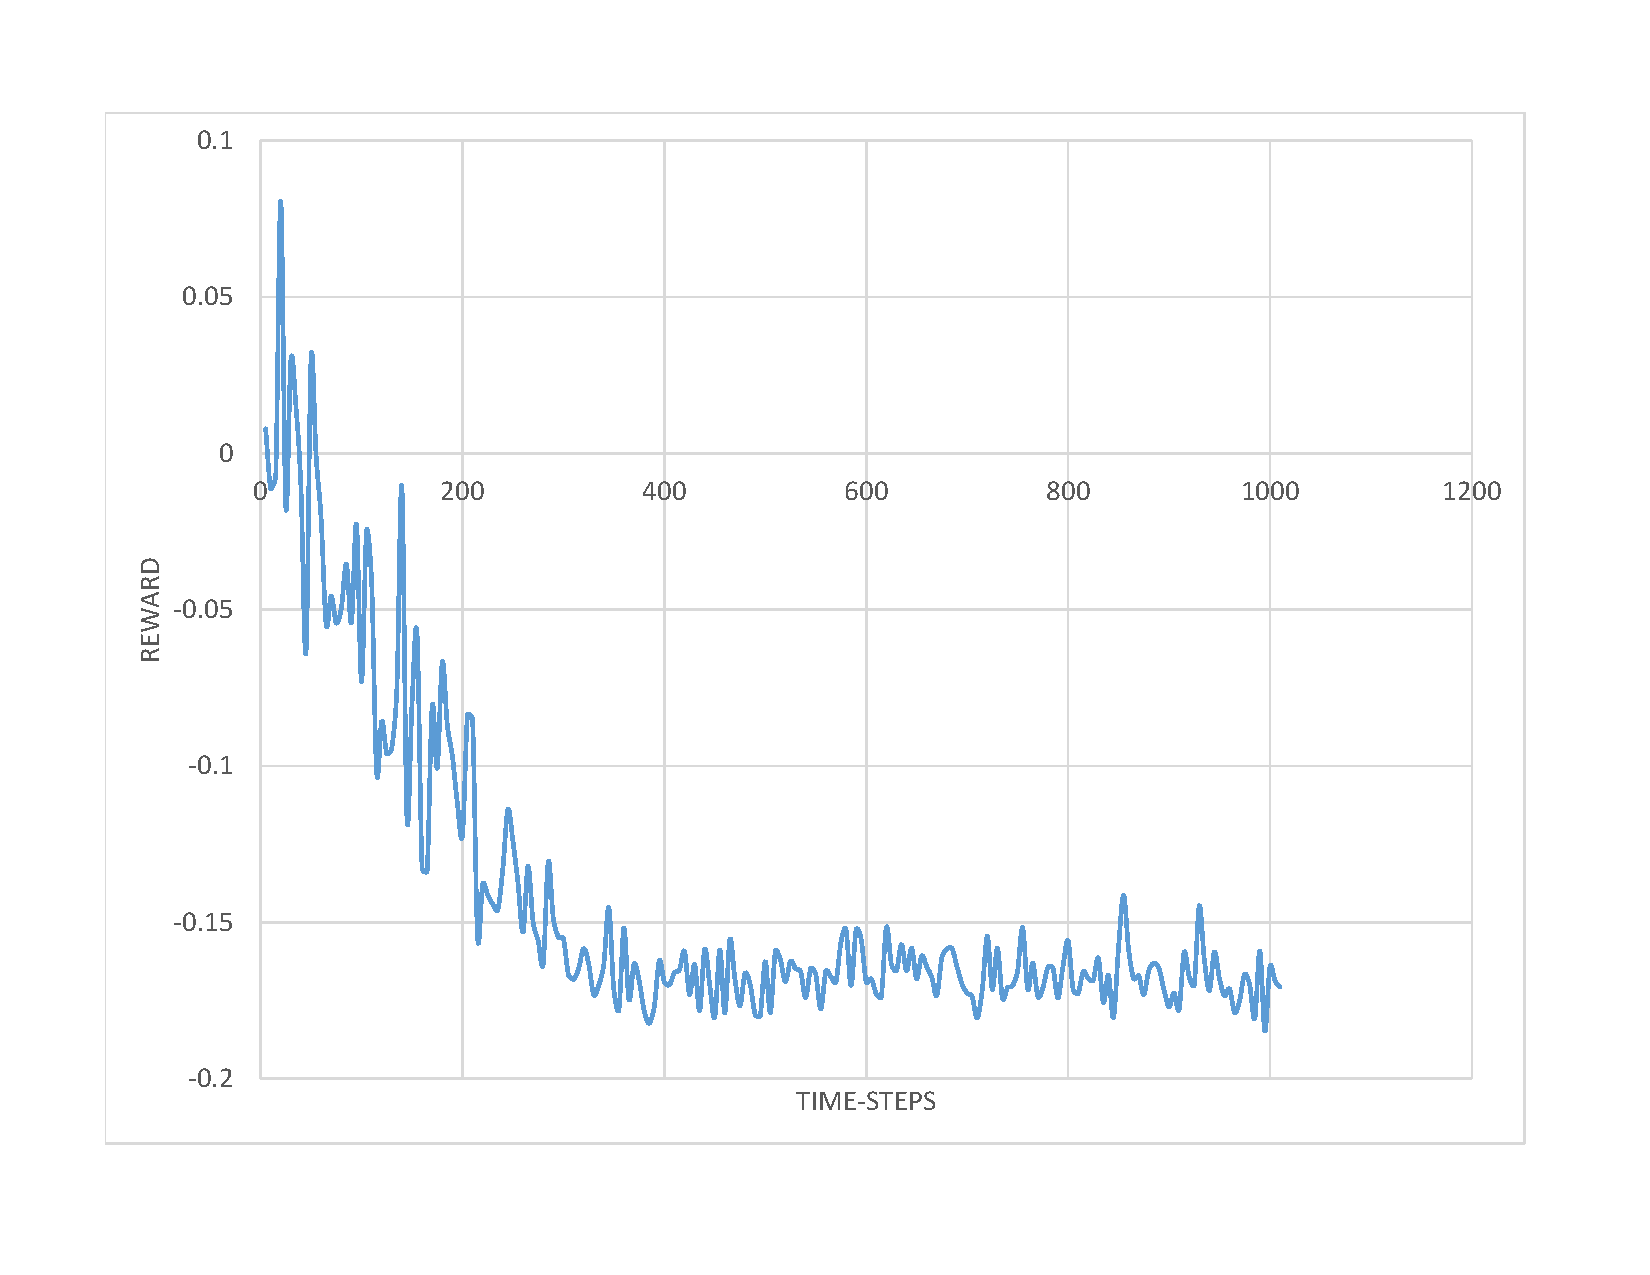
\includegraphics[width=0.8\textwidth]{Figures/ContinuousLoss1}
	\caption{The accumulated Reward for the continuous actions space}
	\label{fig:ContinuousLoss1}
\end{figure}
\begin{figure}[H]
	\centering
	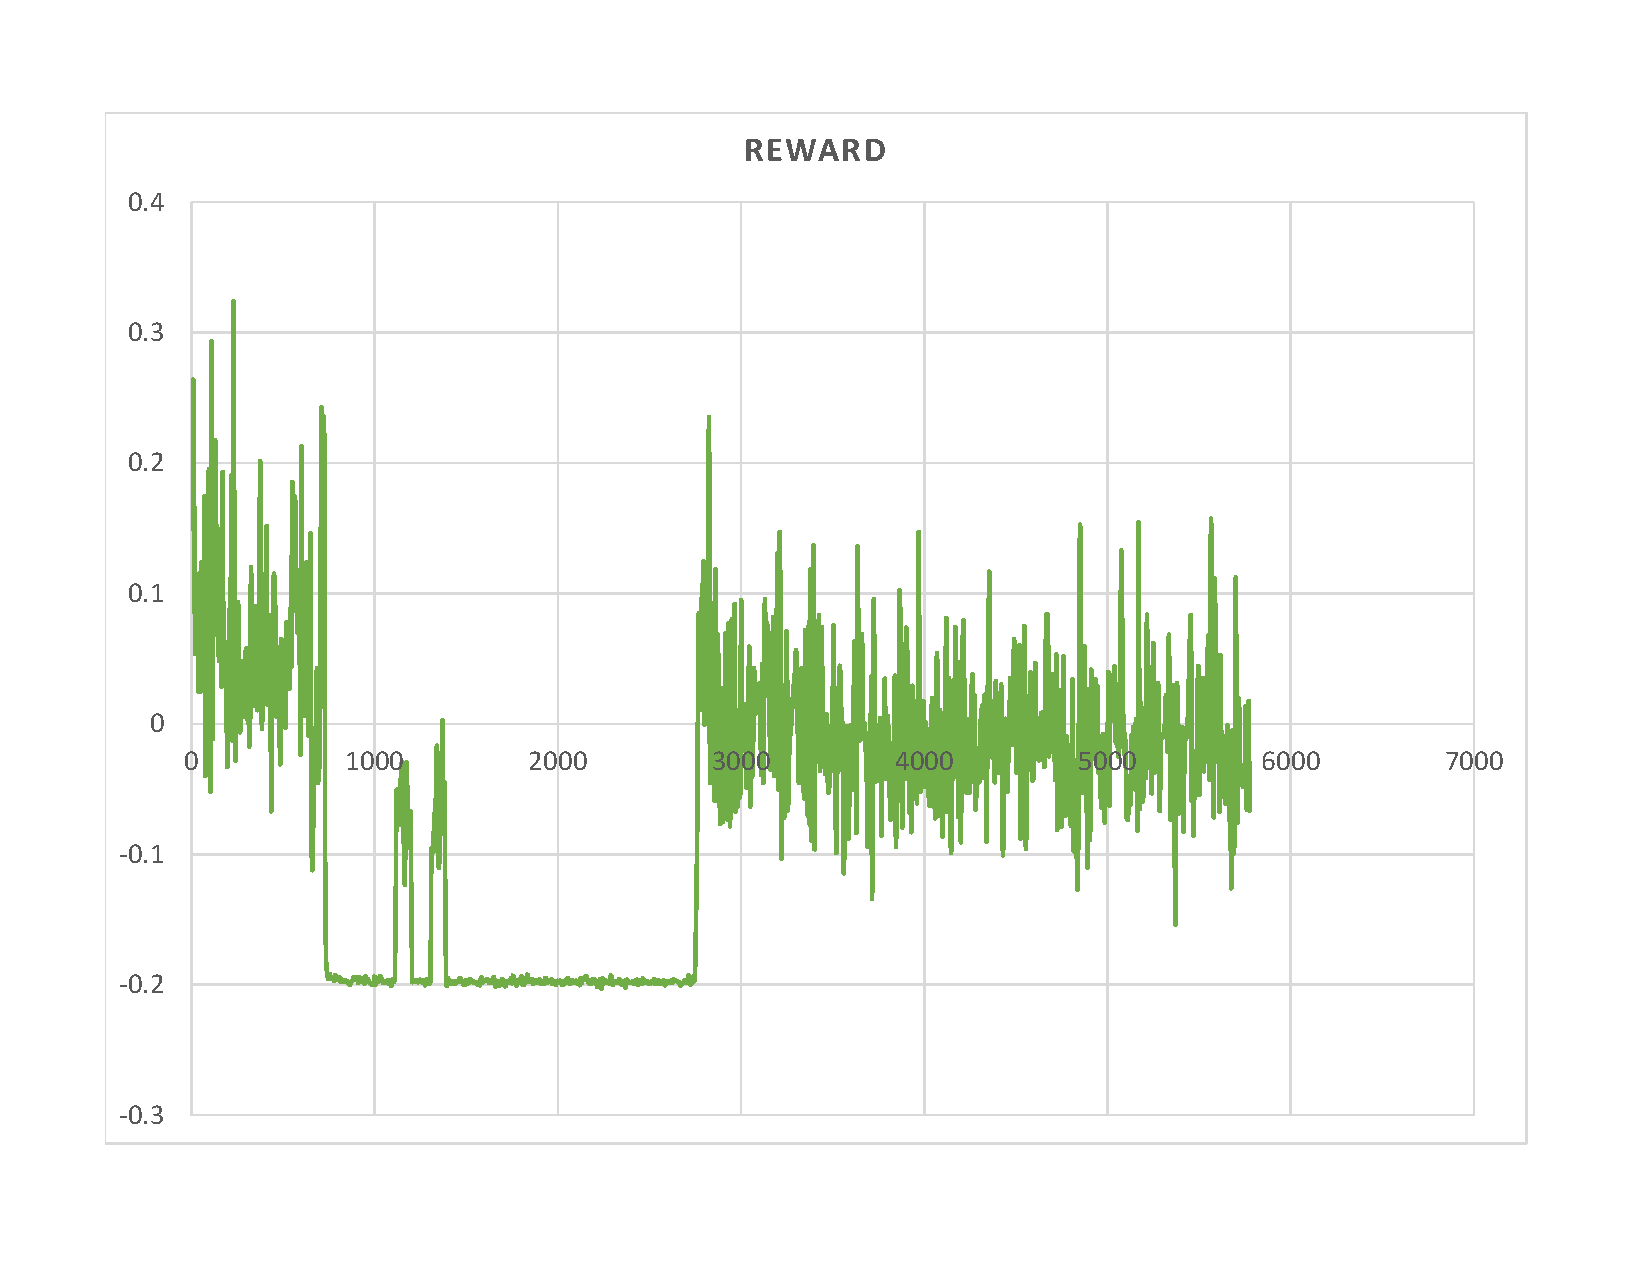
\includegraphics[width=0.8\textwidth]{Figures/ContinuousLoss2}
	\caption{The accumulated Reward for the continuous actions space with a different Loss calculation}
	\label{fig:ContinuousLoss2}
\end{figure}

It is hard to debug or see what is actually happening in the ANN or whether the calculations are right at a specific time, and also these programs do not fire an error in such situations. Therefore these kind of problems are hard to fix. Further investigations are required to find the root problem of malfunctioning in the continuous case.

The DDPG project outlined in \ref{DDPG} section implemented a continuous actions space in a very simplistic way, and it didn't use the principles of estimated variance and mean for making normal distribution, the way it was suggested in \cite{Sutton}. It, instead, used a single layer with the tanh activation function for generating an action with a value between [-1, 1]. This idea might work and would be good to try it for the A3C TORCS.